\documentclass[a4paper,9pt,twocolumn,twoside,]{pinp}

%% Some pieces required from the pandoc template
\providecommand{\tightlist}{%
  \setlength{\itemsep}{0pt}\setlength{\parskip}{0pt}}

% Use the lineno option to display guide line numbers if required.
% Note that the use of elements such as single-column equations
% may affect the guide line number alignment.

\usepackage[T1]{fontenc}
\usepackage[utf8]{inputenc}

% pinp change: the geometry package layout settings need to be set here, not in pinp.cls
\geometry{layoutsize={0.95588\paperwidth,0.98864\paperheight},%
  layouthoffset=0.02206\paperwidth, layoutvoffset=0.00568\paperheight}

\definecolor{pinpblue}{HTML}{185FAF}  % imagecolorpicker on blue for new R logo
\definecolor{pnasbluetext}{RGB}{101,0,0} %



\title{Creating a Kidney Transplant Risk Calculator using GEO datasets (Group
24)}

\author[]{460352996 470066919 480145820 480407614}

  \affil[]{GitHub code repository is
\href{https://github.sydney.edu.au/aauw2900/DATA3888FinalProject}{here}}

\setcounter{secnumdepth}{0}

% Please give the surname of the lead author for the running footer
\leadauthor{460352996 470066919 480145820 480407614}

% Keywords are not mandatory, but authors are strongly encouraged to provide them. If provided, please include two to five keywords, separated by the pipe symbol, e.g:
 \keywords{  Obesity |  Regression |  Correlation |  Prediction  }  

\begin{abstract}
Kidney failure is the final stage of renal disease and is dangerous for
the body as the excretory system fails to function properly. Therefore
medical intervention in the form of renal dialysis or organ
transplantation is required. Organ transplantation is a lifesaving
treatment for those people diagnosed with Kidney disease and is greatly
preferred over renal dialysis. It has the potential to offer a better
quality of life for the patient - fewer health problems and reduced
restrictions on diet- to name a few benefits. Despite the benefits,
organ allocation has posed itself as a major resource balance problem.
This shortage in donor kidneys results in the need for a careful
assessment in allocating organs to patients that potentiate in maximal
survival time. We propose a tool that can aid in the effective and
accurate allocation of these organs.
\end{abstract}

\dates{This version was compiled on \today} 

% initially we use doi so keep for backwards compatibility
% new name is doi_footer

\pinpfootercontents{A Research on Kidney Transplant}

\begin{document}

% Optional adjustment to line up main text (after abstract) of first page with line numbers, when using both lineno and twocolumn options.
% You should only change this length when you've finalised the article contents.
\verticaladjustment{-2pt}

\maketitle
\thispagestyle{firststyle}
\ifthenelse{\boolean{shortarticle}}{\ifthenelse{\boolean{singlecolumn}}{\abscontentformatted}{\abscontent}}{}

% If your first paragraph (i.e. with the \dropcap) contains a list environment (quote, quotation, theorem, definition, enumerate, itemize...), the line after the list may have some extra indentation. If this is the case, add \parshape=0 to the end of the list environment.


\hypertarget{introduction}{%
\subsection{Introduction}\label{introduction}}

Excess weight is the new epidemic of the 21st century and has resulted
in many significant health and economic consequences for the global
population (Stein and Colditz, 2004). In Australia, the obesity epidemic
has spread drastically as 1 in 3 adults are classified as overweight or
obese (Australian Institute of Health and Welfare, 2019). Researches
have shown that this epidemic is more common in males than females and
hence, BYU Human Performance Research Centre has collected data from 250
men of various age and obtained estimates of the percentage of body fat
through underwater weighing and various body circumference measurements
(Rahman and Harding, 2013; DASL, n.d.). As body fat percentage is
difficult to calculate in real life, the value for body fat percentage
was derived from body density using the Siri's 1956 equation (DASL,
n.d.).

\hypertarget{objective}{%
\subsection{Objective}\label{objective}}

Our main objective is to create a risk calculator that can assist
practitioners in their decision making for patient kidney allocation and
inform prescriptions for immunosuppressive drugs. Firstly, our
calculator will utilise patient's genetic expression from RNA-Seq to
predict the chance of them experiencing T-cell/antibody mediated acute
rejection, which is a sudden decline in graft function. This can help
practitioners in deciding whether more aggressive immune suppression
methods are required to prevent rejection. We will then estimate the
probability until donor specific antibodies arise for the patient
phenotype, based upon potential numbers of eplet mismatches they could
have with donor kidneys. DSA presence has been found to be associated
with many forms of rejection and graft failure. A way to minimise graft
dysfunction is for the patient to take immunosuppressive drugs, which as
a consequence could increase their risk of contracting diseases.
However, some rare patients are found to be operationally tolerant,
which means that they still maintain stable graft function after removal
of these drugs. Hence, our final part will be assessing the patient's
reliance on immune suppression, which can help with prescription making
for the practitioner.

\hypertarget{target-audience}{%
\subsection{Target Audience}\label{target-audience}}

We believe that our product is best suited for clinical settings that
foster shared decision making between the patient and the nephrologist.
According to Gordan's 2013 paper , Shared Decision Making promotes
patient centered care allowing for the integration of the nephrologist's
expertise on renal allograft dysfunction as well as the patient's values
and beliefs concerning future treatment. Our tool will provide an
opportunity for discussion between the patient and practitioner that
concerns the nature of treatment pre, during and post organ
transplantation.

\hypertarget{risk-calculator}{%
\subsection{Risk Calculator}\label{risk-calculator}}

\hypertarget{predicting-acute-rejection}{%
\subsubsection{1. Predicting acute
rejection}\label{predicting-acute-rejection}}

\hypertarget{data-cleaning-and-processing}{%
\paragraph{1.1. Data cleaning and
processing}\label{data-cleaning-and-processing}}

We combined 3 datasets, DASL Dataset (R10-09) \&
\textgreater{}\textgreater{}\textgreater{}\textgreater{}\textgreater{}\textgreater{}\textgreater{},
to build part one of the risk calculator. For two of the them, we
performed cpm, log2 transformation appropriately and changed ensemble id
to gene symbols. We joined the three datasets based on common gene
symbols and performed quantile normalisation to reduce batch effect.
This allowed more robust predictions that can be generalised to
different sequencing platforms. We performed feature selection based on
differentially expressed genes between stable and acute rejection
patients, using the limma function. The top 100 most significant genes
were selected for a more comprehensive model.

\hypertarget{selecting-a-model}{%
\paragraph{1.2. Selecting a Model}\label{selecting-a-model}}

For model selection, penalised logistic regression models were selected
as they allow output of a specific risk rather than a binary outcome,
and it reduces issues associated with overfitting, thus solving the
large p small n problem. Between ridge, lasso and elastic net , elastic
net was selected as it shows the highest accuracy, a stable AUC, and
small Brier score using cross validation.

\hypertarget{output}{%
\paragraph{1.3. Output}\label{output}}

In our product, the input raw counts will be transformed. If the data
uses ENSEMBL ID, we converted them to official gene symbols. The output
will be a colour coded gauge plot showing both percentage of the
patient's risk and percentage of the population risk of acute rejection.
This visualisation is clear and easy to understand which is suitable for
our target audience.

\hypertarget{limitations}{%
\paragraph{1.4. Limitations}\label{limitations}}

If the input doesn't include the same genes in the model, a new model
will be trained on the spot. However this creates a limitation of the
long computational time.

\hypertarget{estimating-time-to-de-novo-dsa-presence}{%
\subsubsection{2. Estimating Time to de novo DSA
Presence}\label{estimating-time-to-de-novo-dsa-presence}}

\hypertarget{data-cleaning-and-processing-1}{%
\paragraph{2.1. Data cleaning and
processing}\label{data-cleaning-and-processing-1}}

Here we use the data provided by dr Germaine wong to calculate an
estimate predicting the outcome of a graft based on the recipient's
phenotypic information. Based on a study by Dayoub et al.~in 2018 we
choose age and gender as phenotypic predictors for graft survival. Here
we first create a survival object using presence or absence of class 2
de nova DSA's and the number of days for it to form, which is our
dependent variable for our Kaplan Meier curve. here we focused on DSA as
its an established biomarker for predicting antibody-mediated rejection
which in turn is the leading cause of graft loss

\hypertarget{output-1}{%
\paragraph{2.2. Output}\label{output-1}}

The output is a plot estimating the survival probability of a graft
based on the patient's age and gender. As the patient would not know the
proportion of mismatches he/she would have with a particular donor we
stratified the mismatches based on the mean number of mismatches in the
provided data which was 30. This gives the practitioner and the patient
a better idea of what to expect based on what the previous patient with
similar characteristics experienced. Ideally, this can be used in
resource allocation and prescribing medication. Just to highlight, this
is not used as a predictor of graft survival but only a guide.

\hypertarget{limitations-1}{%
\paragraph{2.3. Limitations}\label{limitations-1}}

The main issue was the size of the data set is small. (only 198
entries). So when we stratify it further based on age, gender, and
mismatches we end up with little information for each subgroup.
therefore we don't have enough data to represent the entire
subpopulation fairly, meaning that some curves are uninformative.

\hypertarget{predicting-operational-tolerance}{%
\subsubsection{3. Predicting Operational
Tolerance}\label{predicting-operational-tolerance}}

\hypertarget{data-cleaning-and-processing-2}{%
\paragraph{3.1. Data cleaning and
processing}\label{data-cleaning-and-processing-2}}

To predict operational tolerance, we collected a dataset that contained
raw gene expressions from tolerant patients, and normal patients which
still required immune suppression for graft function. After quantile
normalisation and batch effect removal, we performed feature selection.
Firstly, genes with noticeable counts in at least one groups was
retained by using the edgeR package. We then selected the most
differentially expressed genes between the two groups using multiple
t-tests. Finally, a review by Massart et al. (2017) suggested a
collection of genes that were highly differential between tolerant and
normal patients, and so these were also added to our final training
dataset.

\hypertarget{selecting-a-model-1}{%
\paragraph{3.2. Selecting a Model}\label{selecting-a-model-1}}

Similar to part 1, we performed penalised logistic regression models to
account for possible overfitting in a large p small n situation. Elastic
net once again proved to be a better model than Ridge and LASSO, showing
higher accuracies and AUC after repeated cross-validation.

\hypertarget{output-2}{%
\paragraph{3.3. Output}\label{output-2}}

The output is a simple colour coded gauge plot showing both percentage
of the patient's reliance and percentage of the population requiring
immunosuppression, making it suitable for our target audience.

\hypertarget{limitations-2}{%
\paragraph{3.4. Limitations}\label{limitations-2}}

However, since operational tolerance is rare, only a handful of data
samples are available, making it difficult to diagnose. Also, like Part
1, another limitation of the model is it has to be `retrained' for if
the input does not contain the same genes in the model.

\hypertarget{conclusion}{%
\subsection{Conclusion}\label{conclusion}}

In conclusion, using the Shared decision-making approach for our risk
calculator, we hope both the practitioner and patient are able to make
informed decisions and derive the optimal treatment option. This
includes allocating reliable donor kidneys to the patient and
prescribing the correct dosage of immunosuppressive drugs. In terms of
future work, we need more diverse and larger datasets to account for
variation and possible confounders within the population, and also
increase confidence. For example, the eplet data is made up of mostly
Caucasian patients only. Ultimately, shared decision making should be
implemented more widely within organ transplantation.

\newpage

\hypertarget{reference-list}{%
\subsection{Reference List}\label{reference-list}}

\hypertarget{section}{%
\subsubsection{1.}\label{section}}

Dayoub, J.C. Cortese, F., Anzic, A, 2018, The Effects of Donor Age on
Organ transplants: a review and implications for aging research,
Experimental Gerontology, Vol 110, pp.~230-240, Retrieved from
\textless{}\textgreater{}

\hypertarget{section-1}{%
\subsubsection{2.}\label{section-1}}

Dorr, C. R., Oetting, W. S., Jacobson, P. A., \& Israni, A. K. (2018).
Genetics of acute rejection after kidney transplantation. Transplant
International, 31(3), 263-277.

\hypertarget{section-2}{%
\subsubsection{3.}\label{section-2}}

Edgar R., Domrachev M., Lash AE. (2002). Gene Expression Omnibus: NCBI
gene expression and hybridization array data repository. Nucleic Acids
Res, 30(1),207-10.

\hypertarget{section-3}{%
\subsubsection{4.}\label{section-3}}

Gordon, E.J., 2013, Opportunities for Shared Decision Making in Kidney
Transplantation, American Journal of Transplantation, Vol.13, no.5
pp.~1149-1158.

\hypertarget{section-4}{%
\subsubsection{5.}\label{section-4}}

Kleinbaum, D.G., 2005 Klein, M., `Introduction to Survival Analaysis' in
Survival Analysis: A self learning text, Springer, New York, NY pp.1-43.

\hypertarget{section-5}{%
\subsubsection{6.}\label{section-5}}

Massart, A., Ghisdal, L., Abramowicz, M., \& Abramowicz, D. (2017).
Operational tolerance in kidney transplantation and associated
biomarkers. Clinical \& Experimental Immunology, 189(2), 138-157.

\hypertarget{section-6}{%
\subsubsection{7.}\label{section-6}}

Tambur, A.R. 2018, HLA-epitope Matching or Eplet Risk Stratification:
The Devil is in the Details, Front Immunol, Vol.9

\hypertarget{appendixes}{%
\subsection{Appendixes}\label{appendixes}}

\hypertarget{appendix-a}{%
\subsubsection{Appendix A}\label{appendix-a}}

Kaplan-Meier curve: Estimated Probability for Class II de novo DSA
Appearance

\begin{center}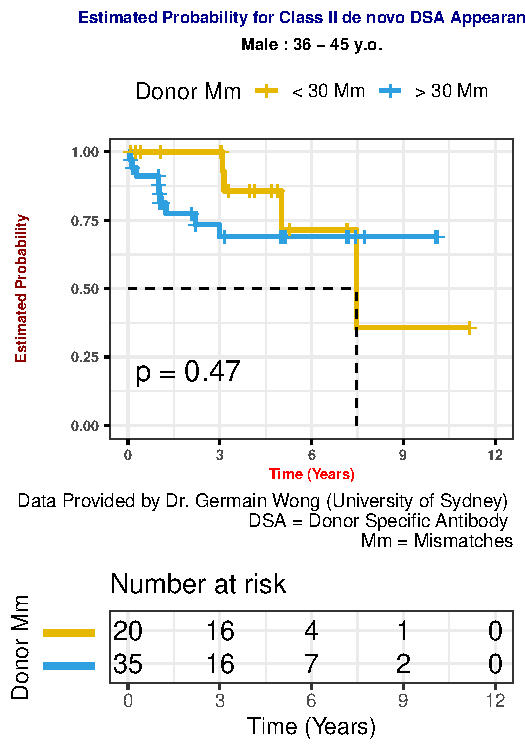
\includegraphics{Executive_Report_files/figure-latex/eplet-1} \end{center}

\hypertarget{appendix-b}{%
\subsubsection{Appendix B}\label{appendix-b}}

Penalised Logistic Regression: Risk of Acute Rejection

\hypertarget{appendix-c}{%
\subsubsection{Appendix C}\label{appendix-c}}

Penalised Logistic Regression: Reliance on Immunosuppression

%\showmatmethods


\bibliography{pinp}
\bibliographystyle{jss}



\end{document}

